\subsection{Leitungsbeläge} % (fold)
\label{sub:leitungsbel_ge}

	Alle für die Signalübertragung relevanten Eigenschaften der Leitung lassen sich in einer Vierpolschaltung als Ersatzschaltbild darstellen. 
	Dabei werden die Größen wie Induktivität, Kapazität und Widerstand jeweils nur für ein kurzes (infinitesimales) Leiterstück l = dx betrachtet, in dem sie als konstant angenommen werden können. 
	Ändern sich diese Größen über die gesamte Leitung nicht, oder kaum, so spricht man von einer homogenen Leitung, wie sie im Versuch zumeist vorliegen wird.

	\begin{figure}[H]
		\center	
		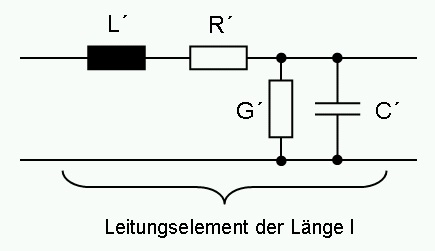
\includegraphics[scale = 0.9]{messwerte/Leitungsbelaege.jpg}
		\caption{\centering Vierpol-Ersatzschalbild eines Leitungsstücks der Länge l = dx \cite{vierpol}} %fick dich schröter!!!
		\label{leitungsbelaege}
	\end{figure}


	\begin{description}
		\item[Widerstandsbelag R':] \hfill\\
			Bezeichnet im wesentlichen den ohmschen Gleichstromwiderstand der Leitung. 
			Teilweise wird in Datenblättern symmetrischer Kabel auch der Schleifenwiderstand eines Adernpaares angegeben. 
			Der Wert des Widerstandsbelags ist in der Regel materialabhängig und steigt mit höheren Frequenzen, da durch den Skineffekt der Strom aus dem Inneren der Leitung in die äußeren Bereiche verdrängt wird und somit die effektiv vom Strom durchgeflossene Fläche kleiner wird. 
			Vergleiche dazu mit:

			\begin{equation}	
				R = \rho \dfrac{A}{L}		
			\end{equation}

		\item[Kapazitätsbelag C':]\hfill\\
			Diese Größe ist hauptsächlich durch den geometrischen Aufbau und die Dielektrizitätskonstante der Isolierung bestimmt. 
			Wie bei der Kapazität  eines Kondensators ist der Wert umso größer, je näher die hin und zurückführenden Adern bei einander liegen und nimmt mit größerer Leiteroberfläche zu. 
			Leitungen hoher Güte haben kleinere Werte für C'.

		\item[Induktivitätsbelag L':]\hfill\\
			Der Wert setzt sich aus einem äußeren und einem inneren Induktivitätsbelag zusammen. 
			Der äußere Induktivitätsbelag ist vom geometrischen Leitungsaufbau und von den magnetischen Eigenschaften des Leiters abhängig. 
			Da normalerweise keine ferromagnetischen Leiter verwendet werden, ist der Induktivitätsbelag unabhängig vom Stromfluss. 
			Ein viel kleinerer innerer Induktivitätsbelag beruht auf den magnetischen Wechselfeldern im Leiter. 
			Dieser Wert nimmt bei höhen Frequenzen weiter ab, da infolge des Skineffekts das Leiterinnere feldfrei wird. 
			In guter Näherung kann dieser Anteil daher vernachlässigt und der Induktivitätsbelag als frequenzunabhängig angesehen werden.

		\item[Ableitungswiderstand G':]\hfill\\
			In diesem Wert werden Isolationsverluste und die dielektrischen Verluste der Isolierung erfasst. 
			Der Ableitungswiderstand ist vom Isolationsmaterial und der Frequenz abhängig. 
			Sein Wert ist im allgemeinen recht groß und daher wird oft sein Kehrwert, die Leitfähigkeit in mS/km oder $\mu$S/m angegeben.
	\end{description}

	\cite{unterlagen}

% subsection leitungsbel_ge (end)


\subsection{Wellenwiderstand} % (fold)
\label{sub:wellenwiderstand}

	Der Wellenwiderstand $Z_L$ ist der Widerstand, den eine Leitung der Ausbreitung einer elektromagnetischen Welle entgegenbringt.
	$Z_L$ wird benötigt um Reflexionen der übertragenen Signale an Schnittstellen zu verhindern (siehe Anpassung).

	\begin{equation}			
		Z_L = \sqrt{\dfrac{R' + i \omega L'}{G' + i \omega C'}}		
	\end{equation}

	Für große Frequenzen, wie sie im Versuch vorliegen, lässt sich die Gleichung unter Vernachlässigung von G' und R' vereinfachen zu:

	\begin{equation}			
		Z_L = \sqrt{\dfrac{L'}{C'}}		
	\end{equation}

	$Z_L$ lässt sich durch Ausmessen der Induktivitäts- und Kapazitätsbeläge mit einer LC- Brücke durch 2 Messungen bei höherer Frequenz bestimmen. 
	Die Wellenlänge muss aber dennoch sehr viel größer als die Kabellänge sein. 
	Die eine Messung erfolgt bei offenem Ende (Leerlauf) und liefert C', für die andere wird das Kabel kurzgeschlossen und man ermittelt L'. 
	Alternativ kann man $Z_L$ aus geometrischen Überlegungen gewinnen:

	Für Koaxialkabel mit D als Durchmesser der äußeren Leitung und d als inneren Durchmesser gilt in etwa:

	\begin{equation}		
		Z_L = \dfrac{60 \Omega}{\sqrt{\varepsilon_r}} \cdot \ln \left(\dfrac{D}{d}\right)		
	\end{equation}

	Für Zweidrahtleitungen der Dicke d mit Adernabstand D kann $Z_L$ abgeschätzt werden als:

	\begin{equation}			
		Z_L = 120 \Omega \cdot \ln\left(\dfrac{D}{d}\right)		
	\end{equation}

	\cite{unterlagen}

% subsection wellenwiderstand (end)

\subsection{Leitungsarten} % (fold)
\label{sub:leitungsarten}

	\subsubsection{Lecherleitung, Zweidrahtleitung, Twisted Pair} % (fold)
	\label{ssub:lecherleitung_zweidrahtleitung_twisted_pair}
	
		Zweidraht- und Lecherleitung bilden die einfachste Leitungsform. 
		Die Lecherleitung als „Urform“ der Leitung geht auf den österreichischen Physiker Ernst Lecher zurück, der mit ihrer Hilfe stehende Wellen in Leitungen untersuchte. 
		Die Twisted Pair Variante besteht aus 2 in einander verdrillten Leitern, wodurch sie einen besseren Schutz gegen Störfelder und Induktionen haben, oft werden sie noch zusätzlich ummantelt. 
		Sie sind heute die am häufigsten verwendeten Leitungstypen bei der Signalübertragung in Computernetzwerken.

		\begin{figure}[H]
			\center
			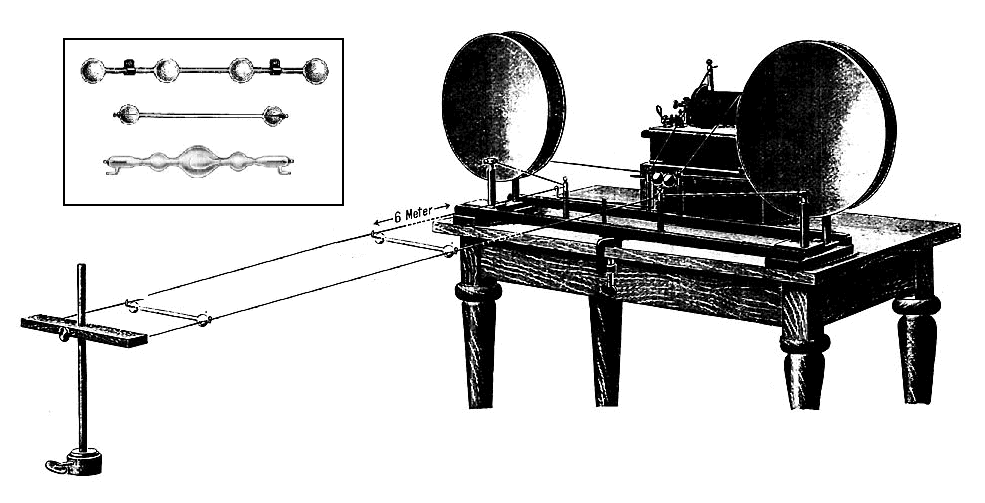
\includegraphics[scale = 0.3]{messwerte/Early_Lecher_line.png}
			\caption{\centering Skizze einer historischen Lecherleitung zur Untersuchung der Spannungsverteilung auf Leitungen bei hohen Frequenzen \cite{lecher}} %fick dich schröter!!!
			\label{Early_Lecher_line}
		\end{figure}

		\begin{figure}[H]
			\center
			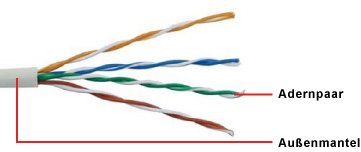
\includegraphics[scale = 0.6]{messwerte/twisted_pair.jpg}
			\caption{\centering Typische Twisted Pair Kabel zur Informationsübertragung in Computersystemen \cite{twisted}} %fick dich schröter!!!
			\label{twisted pair}
		\end{figure}

	% subsubsection lecherleitung_zweidrahtleitung_twisted_pair (end)

	\subsubsection{Koaxialleitung} % (fold)
	\label{ssub:koaxialleitung}
	
		Auch als selbst abschirmende Kabel bezeichnet bilden sie neben den Twisted Pair die zweit häufigste Kabelart in der Hochfrequenztechnik. 
		Etwas komplizierter im Aufbau haben sie viele entscheidende Vorteile gegenüber anderen Leitungsarten. 
		Sie sind breit einsetzbar von etwa 0 bis 10GHz, weisen mäßige Dämpfung auf und strahlen keine Störfelder ab, da das elektrische Feld vollständig auf das innere des Leiters begrenzt ist.

		\begin{figure}[H]
			\center
			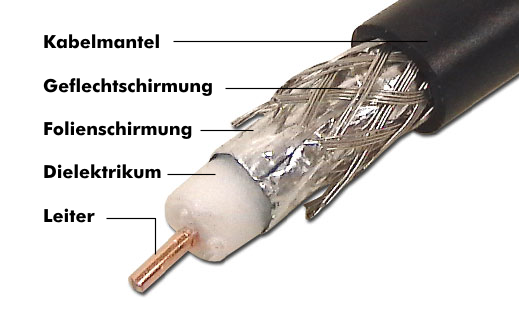
\includegraphics[scale = 0.6]{messwerte/Koaxkabelbild.png}
			\caption{\centering Aufbau eines Koaxialkabels wie es auch im Versuch verwendet wurde \cite{koax}} %fick dich schröter!!!
			\label{Koaxkabelbild}	
		\end{figure}

		Neben den genannten Leitungsarten spielen in der Mikroelektronik noch Streifenleitungen eine Rolle, da sie sich einfach und günstig auf Leiterplatten drucken lassen. 
		Bei sehr hohen Frequenzen (ab ca. 10 GHz) eignen sich Hohlleiter.\cite{unterlagen}

	% subsubsection koaxialleitung (end)

% subsection leitungsarten (end)

\subsection{Verkürzungsfaktor} % (fold)
\label{sub:verk_rzungsfaktor}

	Wie in jedem Medium breiten sich elektromagnetische Wellen auch in Leitern (also in Metallen) langsamer als im Vakuum aus. 
	Die Ausbreitungsgeschwindigkeit $c$ ergibt sich wie aus der Elektrodynamik bekannt zu:

	\begin{equation}		
		c = \dfrac{c_0}{\sqrt{\varepsilon_r \mu_r}}		
	\end{equation}

	Bei den meisten Kabeln ist $\mu_r \approx 1$, deswegen lässt sich die Formel zu

	\begin{equation}		
		c = \dfrac{c_0}{\sqrt{\varepsilon_r}}		
	\end{equation}

	vereinfachen.Die Dielektrizitätskonstante $\varepsilon_r$ ist frequenzabhängig. 
	Mit dem Verkürzungsfaktor $K$ wird das Verhältnis $c/c_0$ bezeichnet, er gibt also auch an, um wie viel sich die Wellenlänge beim Eintritt ins Medium im Vergleich zum Vakuum verkürzt.\cite{unterlagen}

% subsection verk_rzungsfaktor (end)

\subsection{Anpassung und Reflexion} % (fold)
\label{sub:anpassung_und_reflexion}

	Wie in der Gleichstromtechnik ist es für maximale Leistungsübertragung auch in der Hochfrequenztechnik notwendig den Zuleitungswiderstand $Z_L$ dem des Verbrauchers $Z$ anzupassen. 
	Als angepasst bezeichnen wir hier den Zustand wenn $Z_L = Z$ gilt. 
	Die Anpassung ist in der Hochfrequenztechnik aber vor allem deshalb sehr wichtig, da jeder Unterschied der Wellenwiderstände zur Reflexion am Übergang von Kabel zu Verbraucher führt. 
	Diese zurücklaufenden Wellen können den Sender beeinflussen oder wenn die Kabellänge in Größenordnung der Wellenlänge oder darüber liegt, wie es ab dem MHz-Bereich der Fall sein kann, zu stehenden Wellen und großer Verfälschung der vom Sender übertragenen Spannung führen. 
	Um dies zu verhindern muss die Reflexion minimiert werden. Diese errechnet sich nach \cite{buch} zu:

	\begin{equation}	
		r = \dfrac{Z/Z_L - 1}{Z/Z_L + 1}		
	\end{equation}

	Sie wird also minimal gleich Null, wenn Wellenwiderstand $Z_L$ und Eingangswiderstand $Z$ gleich groß sind. \cite{unterlagen}
	Die meisten Hersteller haben sich auf Standartwerte für die Wellenwiderstände von Koaxialleitungen von entweder $50$ oder $75\Omega$ geeinigt. \cite{wikikoax}

% subsection anpassung_und_reflexion (end)

\subsection{Modulation und Mischung} % (fold)
\label{sub:modulation_und_mischung}

	Bei Informationsübertragung mittels elektromagnetischer Wellen ist eine geeignete Modulation des Signals unabdingbar, da die zu übertragenden Nutzfrequenzen meist wesentlich kleiner sind als die mit technischen Mitteln einfach und sauber zu übertragenden Trägerfrequenzen. 
	So ist zum Beispiel beim senden akustischer Signale (Musik, Radio) die Nutzfrequenz im Bereich von 20Hz bis 15kHz, während die optimal mit gebräuchlichen Antennen empfangbaren Frequenzen im Mega- bis Gigahertz-Bereich zu finden sind (siehe Antennenformen). 
	Die bei analoger Signalverarbeitung am häufigsten genutzten Modulationsarten sind Amplituden- und Frequenzmodulation. 
	Wir werden im Versuch nur auf erstere eingehen, da diese leichter umzusetzen und zu messen ist. \\

	
	\subsubsection{Additive Amplitudenmodulation} % (fold)
	\label{ssub:additive_amplitudenmodulation}
	
		Zunächst werden Nutz- und Trägersignal gemischt (addiert). 
		Dies kann z.B. mittels induktiver Kopplung über Transformatoren (Windungsverhältnis 1:1) erfolgen. 
		Das entstehende Signal ist in Abbildung \ref{Mischung} zu sehen:

		\begin{figure}[H]
			\center	
			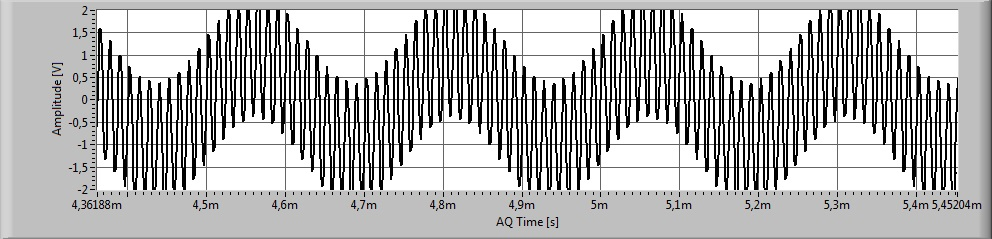
\includegraphics[scale = 0.45]{messwerte/Mischung.jpg}	
			\caption{\centering Mischung zweier Sinussignale mit 5 und 100 kHz und Amplitudenverhältnis 1:0.8, Aufnahme mit LabView-Programm Spektrum-Analyzer(USB6251NI) erstellt} %fick dich schröter!!!	
			\label{Mischung}
		\end{figure}

		Um aus der Mischung eine Modulation zu machen, wird das Signal anschließend an einem Bauteil mit nicht linearer Kennlinie (z.B. exponentiell wie bei einer Diode) verzerrt, wodurch die modulierte Spannung der Form:
		\begin{equation}
			U_{AM} = U_T \sin (\omega_T t) + U_N \sin (\omega_N t) \sin (\omega_T t)
		\end{equation}
		entsteht. Der Plot mit Hilfe von LabView erstellt, ist in Abbildung \ref{AM_addit} zu sehen. Abbildung \ref{FT_AM_addit} zeigt die Fouriertransfomierte:

		\begin{figure}[H]
			\center	
			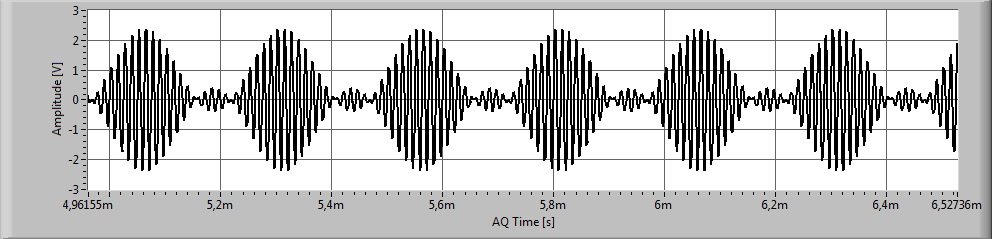
\includegraphics[scale = 0.45]{messwerte/AM_addit.jpg}	
			\caption{\centering Simulation einer additiven Amplitudenmodulation der Form $\sin (\omega t) + a \sin (20 \omega t)$ mit f = 5kHz und a = 0.8, Aufnahme mit LabView-Programm Spektrum-Analyzer(USB6251NI) erstellt} %fick dich schröter!!!	
			\label{AM_addit}
		\end{figure}

		\begin{figure}[H]	
			\center	
			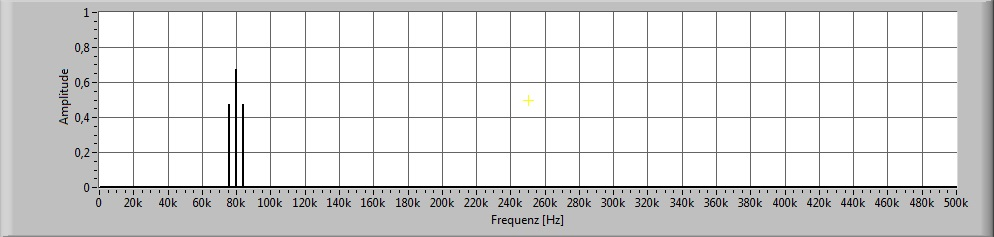
\includegraphics[scale = 0.45]{messwerte/FT_AM_addit.jpg}	
			\caption{\centering Fouriertransformation der additiven Amplitudenmodulation der Form $\sin (\omega t) + a \sin (20 \omega t)$ mit f = 5kHz und a = 0.8, Aufnahme mit LabView-Programm Spektrum-Analyzer(USB6251NI) erstellt} %fick dich schröter!!!	
			\label{FT_AM_addit}	
		\end{figure}

		Wie in Abbildung \ref{FT_AM_addit} zu erkennen, besteht das Spektrum aus der eigentlichen Trägerfrequenz $f_T$ sowie den beiden Seitenbändern die sich wie bei einer Schwebung im Abstand von $\pm f_N$ befinden. 
		Sind die Amplituden des ursprünglichen Nutz- und Trägersignals gleich groß, so geht die Amplitude der Modulierten Spannung periodisch auf 0. 
		Man spricht dann von vollständig durchmodulierten Signalen. 
		Eine prinzipielle Schaltung zur Modulation bzw. Demodulation ist unter Versuchsaufbau und Durchführung zu sehen. \cite{unterlagen}

	% subsubsection additive_amplitudenmodulation (end)

	\subsubsection{Multiplikative Amplitudenmodulation} % (fold)
	\label{ssub:multiplikative_amplitudenmodulation}
	
		Diese Variante wird in der Praxis häufiger eingesetzt. Die Trägerfrequenz wird nicht mit erzeugt und andere unerwünschte Nebenfrequenzen werden unterdrückt. Mathematisch lässt sich die modulierte Spannung wie folgt beschreiben:
		\begin{equation}
			U_{AM} = U_N\sin (\omega_N t)\cdot U_T\sin(\omega_T t)
		\end{equation}
		Folgender Plot wurde zusammen mit der Fouriertransformation durch das LabView Programm +Spektrum-Analyzer(USB6251NI) erstellt:

		\begin{figure}[H]	
			\center	
			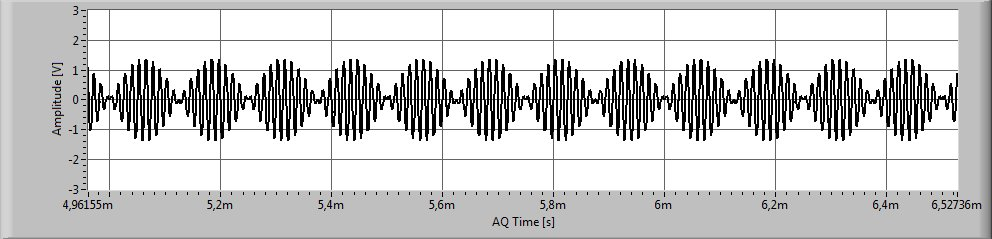
\includegraphics[scale = 0.35]{messwerte/multi.jpg}
			\caption{\centering Simulation einer multiplikativen Amplitudenmodulation der Form $\sin (\omega t) \cdot a \sin (20 \omega t)$ mit f = 5kHz und a = 0.8, Aufnahme mit LabView-Programm Spektrum-Analyzer(USB6251NI) erstellt} %fick dich schröter!!!	
			\label{multi}	
		\end{figure}

		\begin{figure}[H]	
			\center	
			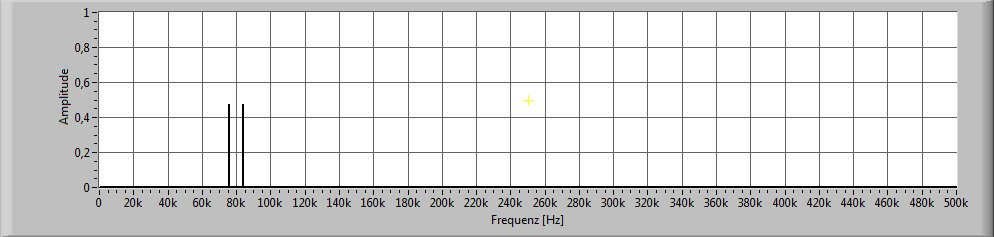
\includegraphics[scale = 0.35]{messwerte/ft-multi.jpg}	
			\caption{\centering Fouriertransformation der multiplikativen Amplitudenmodulation der Form $\sin (\omega t) \cdot a \sin (20 \omega t)$ mit f = 5kHz und a = 0.8, Aufnahme mit LabView-Programm Spektrum-Analyzer(USB6251NI) erstellt} %fick dich schröter!!!	
			\label{ft_multi}	
		\end{figure}

		Wie bei einer Schwebung sind in Abbildung \ref{ft_multi} nur die beiden Seitenbänder zu sehen, der Abstand zwischen ihnen entspricht der doppelten Nutzfrequenz. Zur Realisierung der multiplikativen AM kann ein Diodenringmodulator verwendet werden. Der Prinzipielle Aufbau ist in Abbildung \ref{circuit} zu sehen.\cite{unterlagen}

		\begin{figure}[H]	
			\center	
			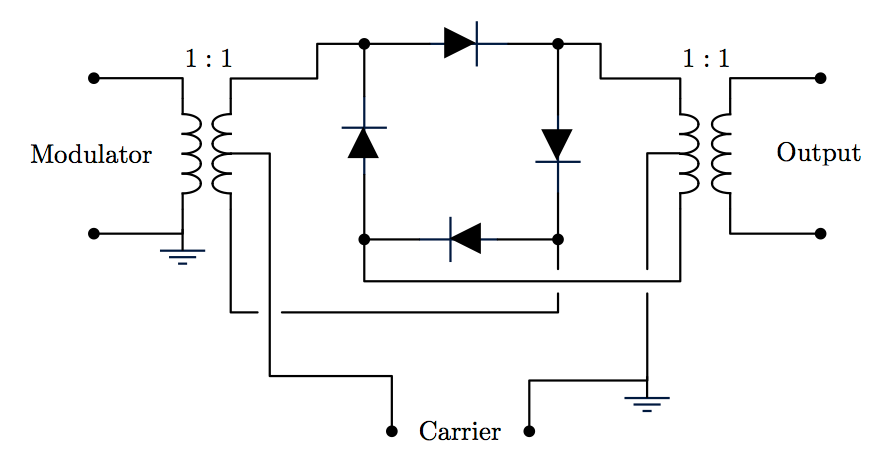
\includegraphics[scale = 0.35]{messwerte/circuit_diagram_parker.png}
			\caption{\centering Schaltung eines Diodenringmodulators zur Realisierung einer multiplikativen Amplitudenmodulation \cite{circuitpic}} %fick dich schröter!!!	
			\label{circuit}	
		\end{figure}

	% subsubsection multiplikative_amplitudenmodulation (end)

% subsection modulation_und_mischung (end)

\subsection{Elektromagnetische Wellen im freien Raum} % (fold)
\label{sub:antennen_und_elektromagnetische_wellen_im_freien_raum}

	Die Ausbreitung der elektromagnetischen Wellen ist die Grundlage jeder Funkanwendung.
	Im geschlossenen Schwingkreis konzentriert sich der Energieaustausch zwischen den Bauteilen.
	Man geht von einem geladenen Kondensator aus, der sich in die Spule entlädt. Durch den
	Entladestrom baut sich im Kondensator das elektrische Feld ab dafür aber das magnetische Feld in
	der Spule auf. Bedingt durch die Selbstinduktion der Spule entsteht wieder eine Ladespannung die
	zum Aufladen des Kondensators führt und somit den Ursprungszustand wiederherstellt.
	Die Wechselwirkung zwischen elektrischem und magnetischem Feld nennt man Elektromagnetische Schwingungen.
	Ein offener Schwingkreis kann als ein „aufgeklappter“ Schwingkreis verstanden werden. 
	Hierbei bilden die Kondensatorplatten den oberen und unteren Abschluss, die Spule befindet sich in der Mitte. 
	Der schematische Übergang ist in Abbildung \ref{schwingkreis_antenne} zu sehen. \cite{unterlagen}

	\begin{figure}[H]	
		\center	
		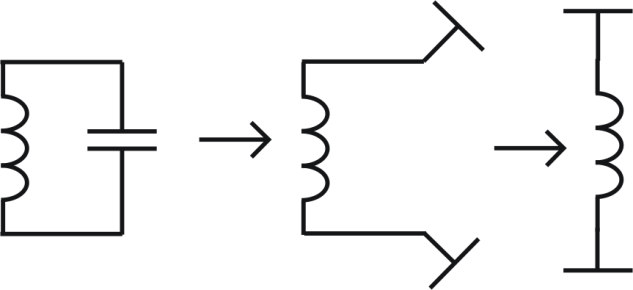
\includegraphics[scale = 0.35]{messwerte/schwingkreis-antenne.png}
		\caption{\centering Schema des Übergangs eines Schwingkreis zur Antenne \cite{unterlagen}} %fick dich schröter!!!	
		\label{schwingkreis_antenne}	
	\end{figure}

	Reduziert man nun die Windungen sowie die Plattengröße, so geht der offene Schwingkreis schließlich in die Antenne über. 
	Die einfachsten Antennenformen sind der $\lambda/2$-Dipol und die Marconi-Antenne. 
	Beim $\lambda/2$-Dipol wird die Spannung in der Mitte angelegt, es bildet sich im günstigsten Fall bei richtiger Frequenz eine stehende Welle aus, mit Strommaximum in der Mitte und Spannungsmaxima an den Enden. 
	Hierfür darf die abgestrahlte Wellenlänge maximal doppelt so groß wie die Antenne sein (deswegen $\lambda/2$). 
	In diesem Fall strahlt die Antenne maximal ab. 
	Dieser Zusammenhang ist in Abbildung \ref{schema_antenne_welle} ersichtlich:

	\begin{figure}[H]	
		\center	
		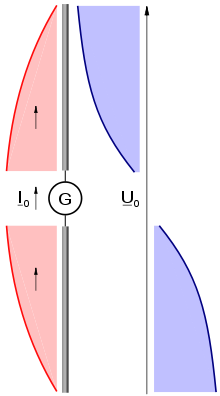
\includegraphics[scale = 0.45]{messwerte/220px-Lineare_antennen_svg.png}
		\caption{\centering Schema zur Entstehung stehender Wellen auf einer $\lambda /2$-Antenne \cite{wave}} %fick dich schröter!!!	
		\label{schema_antenne_welle}	
	\end{figure}

	Der Viertelwellenstrahler oder auch Marconi-Antenne genannt basiert auf dem gleichen Prinzip, nur das eine Hälfte des $\lambda/2$ Dipols entfällt oder durch Erdung bzw. durch mehrere Radials ersetzt wird. 
	Die Strom und Spannungsverteilung ist aber analog zur Halbwellendipolantenne.

% subsection antennen_und_elektromagnetische_wellen_im_freien_raum (end)